\noindent \textred{4.} You want to solve the following three recurrence formulas:
\[
\begin{aligned}
    &A: T(n) = 5T(\frac{n}{2}) + a n \\
    &B: T(n) = T(\frac{n}{3}) + b n^2 \\
    &C: T(n) = 3T(\frac{n}{3}) + c n \log n
\end{aligned}
\]
Can you use Master’s method for each of these? If yes, write down how you check the conditions and the answer. If not, briefly explain why and solve using other methods. \\
(Hint: You may need the harmonic series, i.e. when $n$ is very large, $\log n \approx \sum_{k=1}^n \frac{1}{k})$
\newline \\
\textblue{
$A$: Using Master's Method, $T(n) = a T(\frac{n}{b}) + f(n)$, where $a=5$, $b=2$ and $f(n) = a n$. Therefore, $f(n) = O(n^{\log_b a - \epsilon}) = n^{\log_2 5 - \epsilon}$, where $\epsilon = \log_2 5 - 1 > 0$. So \underline{$T(n) = \Theta(n^{\log_2 5})$}.
\newline \\
$B$: Using Master's Method, $T(n) = a T(\frac{n}{b}) + f(n)$, where $a=1$, $b=3$ and $f(n) = b n^2$. Therefore, $f(n) = \Omega(n^{\log_b a + \epsilon}) = n^{\log_3 1 + \epsilon}$, where $\epsilon = 2 > 0$. Moreover, $\forall c \in [1/9, 1)$, we have $a f(n/b) \leq c f(n)$.
So \underline{$T(n) = \Theta(n^2)$}.
\newline \\
$C$: This recursion can not be solved using Master's method because $f(n) = c n \log n$ is not of exponential form of $n$, thus can not be compared accordingly. Moreover, $\forall \epsilon>0, \log n = O(n^{\epsilon})$. Therefore, we use recursion tree to analyse:
\begin{figure}[!h]
    \centering
    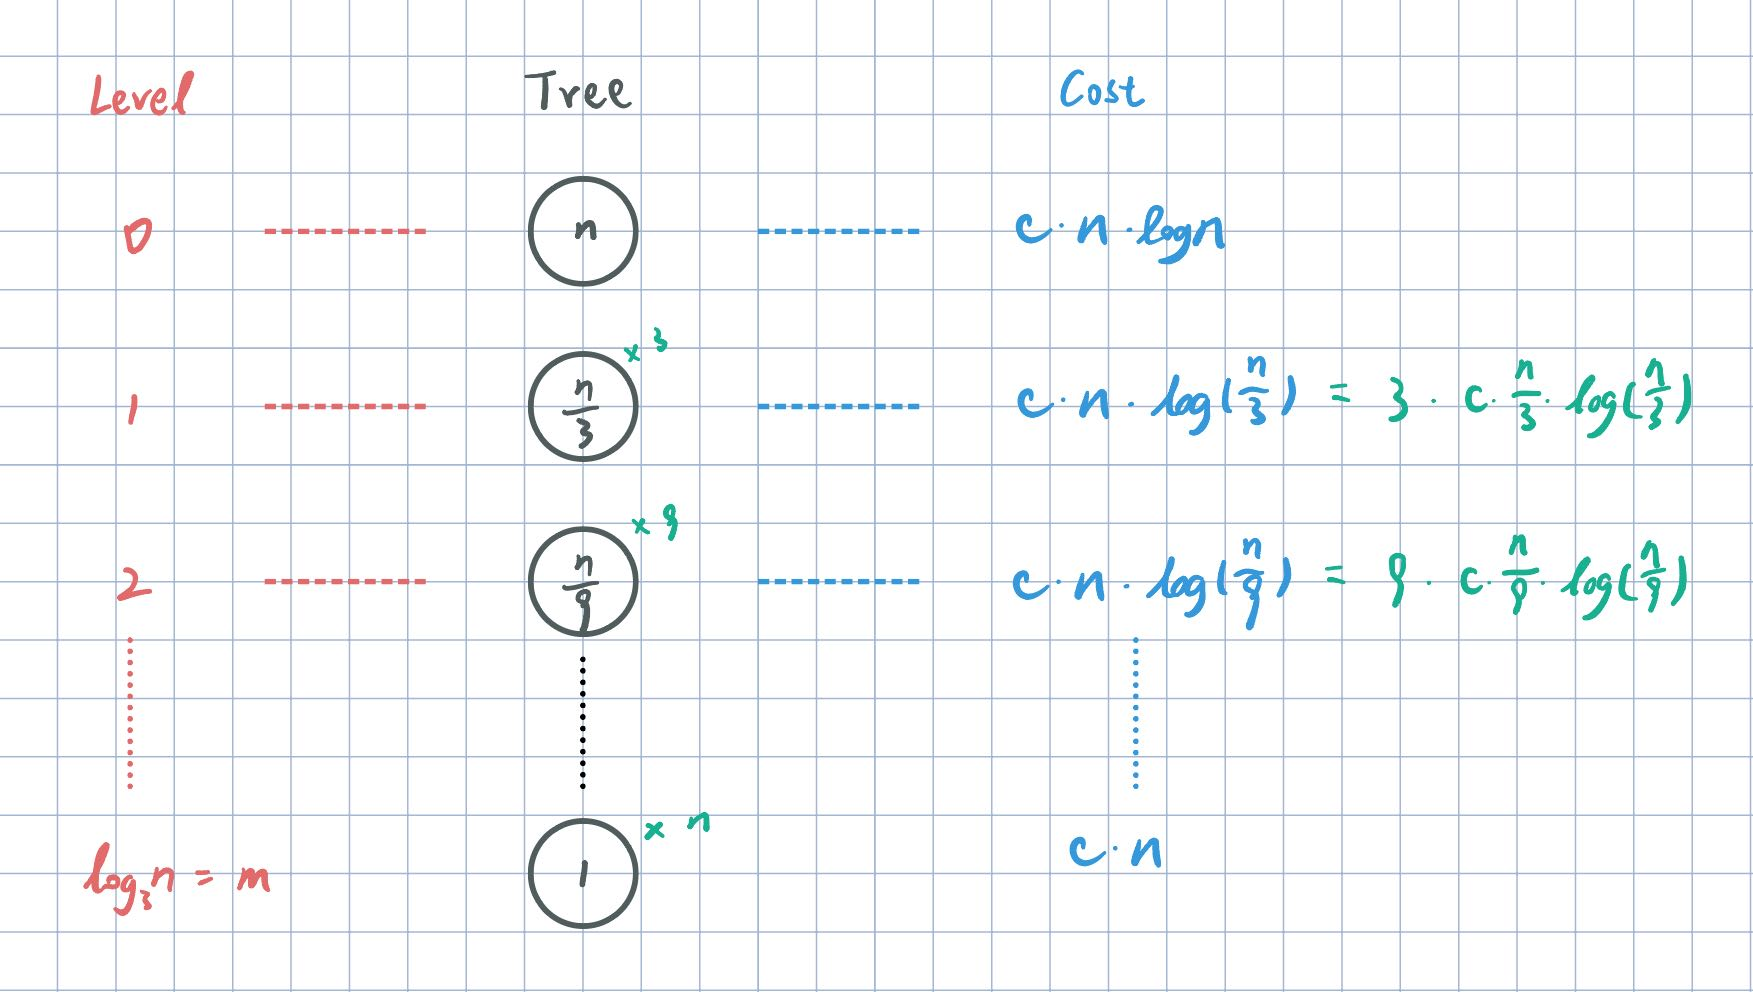
\includegraphics[width=0.7\linewidth]{HWs/HW2/HW02_04.jpg}
    % \label{fig:HW02_01_tree}
\end{figure}
\[
\begin{aligned}
    T(n) &\simeq c \cdot n [\log n + \log (\frac{n}{3}) + \log (\frac{n}{3^2}) + \cdots + \log (\frac{n}{3^{\log_3 n}})]  \\
    &= c \cdot n \sum_{i=0}^{\log_3 n}(\log n - i \cdot \log 3) \\
    &= c \cdot n \log n \log_3 n - c \cdot n \log 3 \cdot \sum_{i=0}^{\log_3 n} i \\
    &= c \cdot n \log n \log_3 n - c \cdot n \log 3 ~\frac{\log_3 n (\log_3 n + 1)}{2} = \underline{\Theta(n(\log n)^2)}
\end{aligned}
\]
}
